\begin{frame}
	\titlepage
\end{frame}


\begin{frame}{Заполнение шаблона}
	\begin{itemize}
		\item Изменить \textbf{config.tex}: имя студента, название предмета и пр. параметры указаны именно там
		\item Заполнить \textbf{content.tex} - файл, который будет содержать весь текст презентации.
		\item Добавить используемую литературу (если есть) в \textbf{refs.bib}. Для удобного поиска источников можно воспользоваться Google Books. Использованные источники можно указывать с помощью команды \textbf{\\cite\{name\_of\_ref\}}
	\end{itemize}
	Далее представлены различные примеры.
\end{frame}

\begin{frame}{Обычный слайд текста}
	Текст сам центрируется по высоте слайда. Центрирование по горизонтали
\end{frame}


\begin{frame}{Список}
	\begin{itemize}
		\item Элемент списка
		      \begin{itemize}
			      \item Элемент вложенного списка
		      \end{itemize}
		\item Элемент списка
		      \begin{enumerate}
			      \item Элементы
			      \item нумерованного
			      \item списка
		      \end{enumerate}
	\end{itemize}
\end{frame}

\begin{frame}{Блоки}
	\begin{exampleblock}{Заголовок блока}
		Текст блока примера. Кстати, ссылка \cite{kingma2014adam}
	\end{exampleblock}

	\begin{alertblock}{}
		Текст блока предупреждения
	\end{alertblock}

\end{frame}

\begin{frame}{Рисунок}
	\begin{figure}[H]
		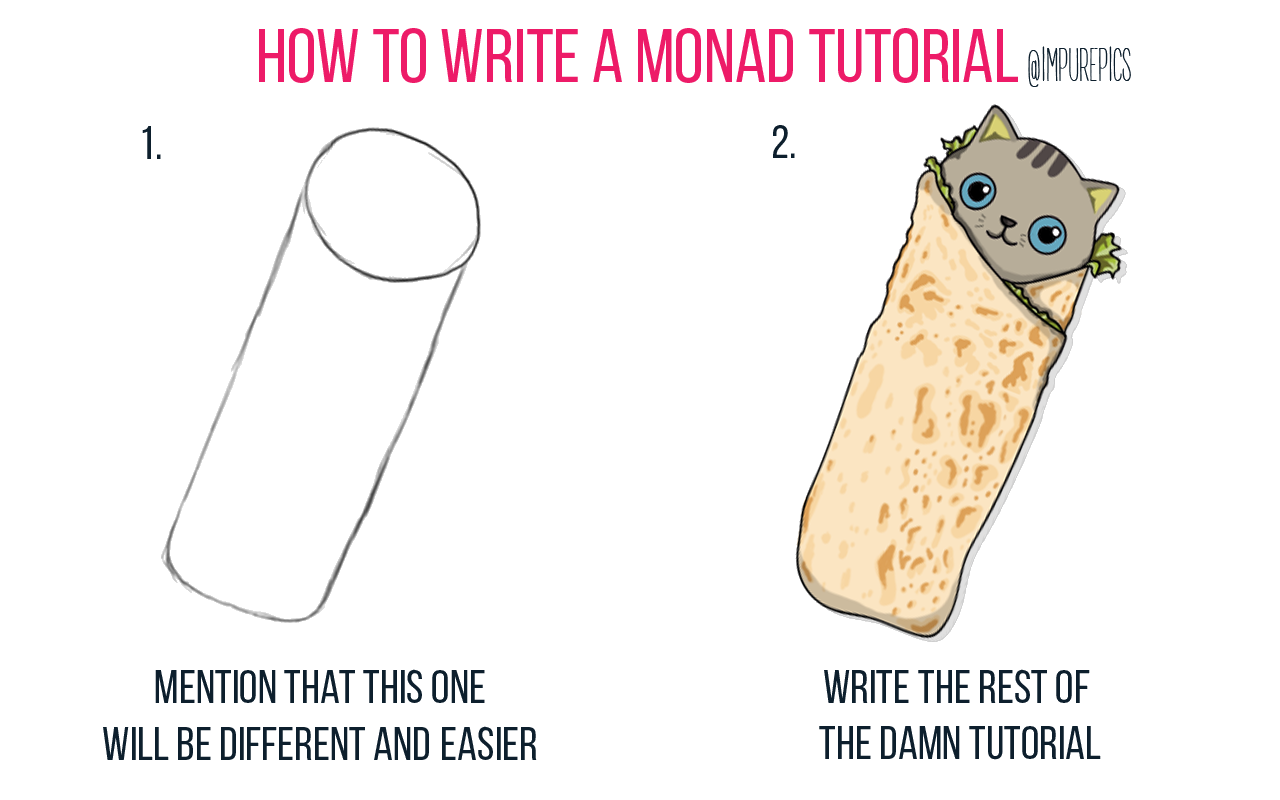
\includegraphics[width=0.5\textwidth]{fig/sample.png}
		\label{fig:sample}
		\caption{Подпись}
	\end{figure}
	\center{\url{https://impurepics.com/}}
\end{frame}

\begin{frame}{Листинг}
	\begin{code}
		\lstinputlisting[language=Haskell]{listings/haskell_code.hs}
		\caption{Да, это опять функциональный код.}
	\end{code}
\end{frame}

\begin{frame}{Формулы, сложна}
	Спектр (спектральная плотность) $\Phi(f)$ в общем случае представляет собой комплексную функцию: $$\Phi(f)=|\Phi(f)|*e^{i\psi(f)}$$
	Модуль этой функции $|\Phi(f)|$ называют спектром амплитуд, а зависимость $\psi(f)$ — спектром фаз.
\end{frame}

\begin{frame}[fragile]{Разбиваем слайд}
	Раз.
	\pause
	Два.
	\pause
	Ну вы поняли.
\end{frame}

\begin{frame}{Анимация?}
	\begin{figure}
		\begin{tabular}{c}
			Но нужен Adobe Reader. Или что-то другое хорошее. \\
			\animategraphics[loop,controls,width=0.9\textwidth]{1}{fig/sgd/descent-}{0}{7}
		\end{tabular}
	\end{figure}
\end{frame}

\begin{frame}{Перечень использованных источников}
	\printbibliography[title=Этот цвет тоже можно поменять.]
\end{frame}
